\section{Idiotenseite}
\subsection{Differentation}

{\setlength{\extrarowheight}{4pt}
	\begin{tabular}{@{}lcl@{}}
		\textbf{f(x)} & $\rightarrow$ & \textbf{f'(x)} \\
		\toprule
		$c$ & $\rightarrow$ & $0$ \\
		$x^n$  & $\rightarrow$ & $n\cdot x^{n-1}$ \\
		$c\cdot g\left(x\right)$  & $\rightarrow$ & $c\cdot g'\left(x\right)$ \\
		$e^x$  & $\rightarrow$ & $e^x$ \\
		$a^x$ & $\rightarrow$ & $a^x\ln(a)$\\
		\midrule
		$g\left(x\right)+h\left(x\right)$  & $\rightarrow$ & $g'\left(x\right)+h'\left(x\right)$ \\
		$u\left(x\right)\cdot v\left(x\right)$  & $\rightarrow$ & $u'\left(x\right)\cdot v\left(x\right)+u\left(x\right)\cdot v'\left(x\right)$ \\ 
		$\frac{u\left(x\right)}{v\left(x\right)}$  & $\rightarrow$ & $\frac{u'\left(x\right)\cdot v\left(x\right)-u\left(x\right)\cdot v'\left(x\right)}{v^2\left(x\right)}$ \\
		$u\left(v\left(x\right)\right)$  & $\rightarrow$ & $u'\left(v\left(x\right)\right)\cdot v'\left(x\right)$ \\
		\midrule
		$\cos\left(x\right)$ & $\rightarrow$ & $-\sin(x)$ \\
		$\sin\left(x\right)$ & $\rightarrow$ & $\cos(x)$ \\	
		$\cosh\left(x\right)$ & $\rightarrow$ & $\sinh(x)$ \\
		$\sinh\left(x\right)$ & $\rightarrow$ & $\cosh(x)$ \\
		$\tan\left(x\right)$ & $\rightarrow$ & $\frac{1}{\cos^2(x)} = 1 + \tan^2(x)$ \\	
		$\ln\left(x\right)$ & $\rightarrow$ & $\frac{1}{x}$ \\
		$f^{-1}\left(x\right) {\scriptscriptstyle (Umkehrf.)}$  & $\rightarrow$ & $\frac{1}{f'(f^{-1}(x))}$ \\
		$\left|x\right|$ & $\rightarrow$ & $\frac{\left|x\right|}{x}$ \\
	\end{tabular}
}

\subsection{Integration}
\begin{center}
	\begin{minipage}{0.2\textwidth}
		\noindent\textbf{Potenzregel} evt Partialbruchzerlegung!
	\end{minipage}%%% to prevent a space
	\begin{minipage}{0.3\textwidth}
		\[ \int x^\alpha = \frac{x^{\alpha  + 1}}{\alpha + 1} + C \]
	\end{minipage}
\end{center}

\begin{center}
	\begin{minipage}{0.2\textwidth}
		\noindent\textbf{Partielle Integration}
	\end{minipage}%%% to prevent a space
	\begin{minipage}{0.3\textwidth}
		\[\int f' \cdot g = f \cdot g - \int f \cdot g'\]
	\end{minipage}
\end{center}

\begin{center}
	\begin{minipage}{0.2\textwidth}
		\noindent\textbf{Allgemeine Substitution}\\
		Wobei $t=g(x)$ und $dt = g'(x)dx$. Siehe An1 ZF
	\end{minipage}%%% to prevent a space
	\begin{minipage}{0.3\textwidth}
		\[\int_{a}^{b} f(g(x)) \cdot g'(x)dx \eqi \int_{g(a)}^{g(b)} f(t) dt\]
	\end{minipage}
\end{center}

\begin{center}
	\begin{minipage}{0.2\textwidth}
		\noindent\textbf{Elementar Substitution}
	\end{minipage}%%% to prevent a space
	\begin{minipage}{0.3\textwidth}
		\[\int f(ax + b)dx = \frac{1}{a}F(ax+b)+C\]
	\end{minipage}
\end{center}

\begin{center}
	\begin{minipage}{0.2\textwidth}
		\noindent\textbf{Exponential allg.}
	\end{minipage}%%% to prevent a space
	\begin{minipage}{0.3\textwidth}
		\[\int e^xdx = e^x + C\]
	\end{minipage}
\end{center}

\begin{center}
	\begin{minipage}{0.2\textwidth}
		\noindent\textbf{Log-Integration}
	\end{minipage}%%% to prevent a space
	\begin{minipage}{0.3\textwidth}
		\[\int \frac{f'(x)}{f(x)} = \ln\left|f(x)\right| + C\]
	\end{minipage}
\end{center}
\subsubsection{Einheitskreis}
\begin{center}
	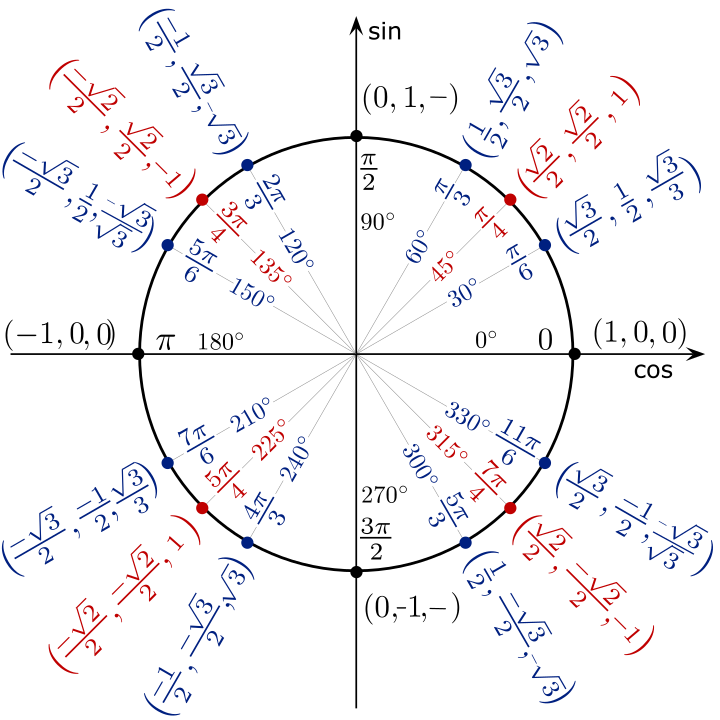
\includegraphics[width=0.8\columnwidth]{Images/einheitskreis}\\
	Punkte auf Kreis [$\cos(\alpha), \sin(\alpha), \tan(\alpha)$]
\end{center}

\subsubsection{Periodizität}
$\cos(a+k\cdot2\pi)=\cos(a) \qquad \sin(a+k\cdot2\pi)=\sin(a) \qquad
(k \in \mathbb{Z})$

\subsubsection{Doppel- und Halbwinkel}	
\begin{align*}
	\sin(2a) &=2\sin(a)\cos(a) &= \frac{2\tan(a)}{1 +\tan^2(a)}\\
	\cos(2a) &=\cos^2(a)-\sin^2(a) &= 2\cos^2(a)-1 &= 1-2\sin^2(a)\\
	\cos^2 \left(\frac{a}{2}\right) &=\frac{1+\cos(a)}{2} \\
	\sin^2 \left(\dfrac{a}{2}\right)&=\frac{1-\cos(a)}{2}
\end{align*}

\subsubsection{Additionstheoreme}
\begin{align*}
	\sin(a \pm b)&=\sin(a) \cdot \cos(b) \pm \cos(a) \cdot \sin(b)\\
	\cos(a \pm b)&=\cos(a) \cdot \cos(b) \mp \sin(a) \cdot \sin(b)\\	
	\tan(a \pm b)&=\dfrac{\tan(a) \pm \tan(b)}{1 \mp \tan(a) \cdot \tan(b)}\\
	\sin(a)+\sin(b) &= 2\sin\left(\frac{a + b}{2}\right)\cos\left(\frac{a - b}{2}\right)\\
	\sin(a)-\sin(b) &= 2\cos\left(\frac{a + b}{2}\right)\sin\left(\frac{a - b}{2}\right)\\
	\cos(a)+\cos(b) &= 2\cos\left(\frac{a + b}{2}\right)\cos\left(\frac{a - b}{2}\right)\\
	\cos(a)-\cos(b) &= -2\sin\left(\frac{a + b}{2}\right)\sin\left(\frac{a - b}{2}\right)\\
	\sin(a)\sin(b)&=\frac{1}{2}(\cos(a-b)-\cos(a+b))\\
	\cos(a)\cos(b)&=\frac{1}{2}(\cos(a-b)+\cos(a+b))\\
	\sin(a)\cos(b)&=\frac{1}{2}(\sin(a-b)+\sin(a+b))\\
\end{align*}

\subsubsection{Potenzen}
\begin{align*}
	\sin^2(a) &= \frac{1}{2}(1 - \cos(2a)) \\
	\sin^3(a) &= \frac{1}{4}(3\sin(a) - \sin(3a)) \\
	\cos^2(a) &= \frac{1}{2}(1 + \cos(2a)) \\
	\cos^3(a) &= \frac{1}{4}(3\cos(a) + \cos(3a)) \\
\end{align*}

\subsection{Vektorgeometrie}
\[\vec{a} \circ \vec{b} = \begin{pmatrix} x_a \\ y_a \\ z_a \end{pmatrix} \circ \begin{pmatrix} x_b \\ y_b \\ z_b \end{pmatrix} = x_a \cdot x_b + y_a \cdot y_b + z_a \cdot z_b\]


\begin{center}	
	\tikzset{ x=1mm, y=1mm }
	\begin{tikzpicture}
		\node {$\vec{a} \times \vec{b} = \begin{pmatrix}
				-2 & 10 \\
				3 & 2 \\
				1 & -1 \\
				-2 & 10 \\
				3 & 2 \\
				1 & -1 \\
			\end{pmatrix} = \begin{pmatrix}
				(\textcolor{blue}{3 \cdot (-1)}) - (\textcolor{red}{1 \cdot 2}) \\
				(\textcolor{blue}{1 \cdot 10}) - (\textcolor{red}{(-2) \cdot (-1)}) \\
				(\textcolor{blue}{(-2) \cdot 2}) - (\textcolor{red}{10 \cdot 3}) \\
			\end{pmatrix} = \begin{pmatrix}
				-5 \\
				8 \\
				-34 \\
			\end{pmatrix}$
		};
		\draw[line width=0.2mm,gray, dashed] (-34,0) -- (-16, 0);
		
		\draw[line width=0.4mm,blue] (-27,6) -- (-23,3);
		\draw[line width=0.4mm,blue] (-27,2) -- (-23,-1);
		\draw[line width=0.4mm,blue] (-27,-2) -- (-23,-5);
		
		\draw[line width=0.4mm,red] (-27,3) -- (-23,6);
		\draw[line width=0.4mm,red] (-27,-1) -- (-23,2);
		\draw[line width=0.4mm,red] (-27,-5) -- (-23,-2);
		
		\draw[line width=0.2mm,black] (-34,11) -- (-16,11);
		\draw[line width=0.2mm,black] (-34,-10) -- (-16,-10);	
	\end{tikzpicture}	
\end{center}
\[
\vec{F}\times \vec{F} = \vec{0}
\]